\documentclass[12pt]{article}
\usepackage{graphicx}
\usepackage{hyperref}
\usepackage[top=2.75in, left=1in, right=1in, bottom=0.25in]{geometry}
\usepackage[utf8]{inputenc}
\usepackage[english]{babel}
\usepackage{fancyhdr}

\setlength{\parindent}{4em}
\setlength{\parskip}{1em}
\pagestyle{fancy}
\fancyhf{}
\rhead{Problem}
\lhead{Huan Huang}
\renewcommand{\headrulewidth}{0.4pt}
\renewcommand{\footrulewidth}{0.4pt}
\rfoot{Page \thepage}

\begin{document}
\begin{titlepage}
	\begin{center}
	\Huge{Web Science cs532-s16}\\
	[0.25in]
	\textsc{\Large Assignment 1 Report}\\
	[4.25in]
	\textsc{\normalsize By: Huan Huang}\\
	\large 01/28/2016\\
	
	
	\end{center}
\end{titlepage}
\newpage

\newgeometry{margin=1in}

\section*{Problem 1}
Demonstrate that you know how to use "curl" well enough to
correctly POST data to a form.  Show that the HTML response that
is returned is "correct".  That is, the server should take the
arguments you POSTed and build a response accordingly.  Save the
HTML response to a file and then view that file in a browser and
take a screen shot.

\subsection*{Answer}
For this problem, I first created a form by using Google Form. Here is a picture of the form.
\begin{figure}[h]
\centering
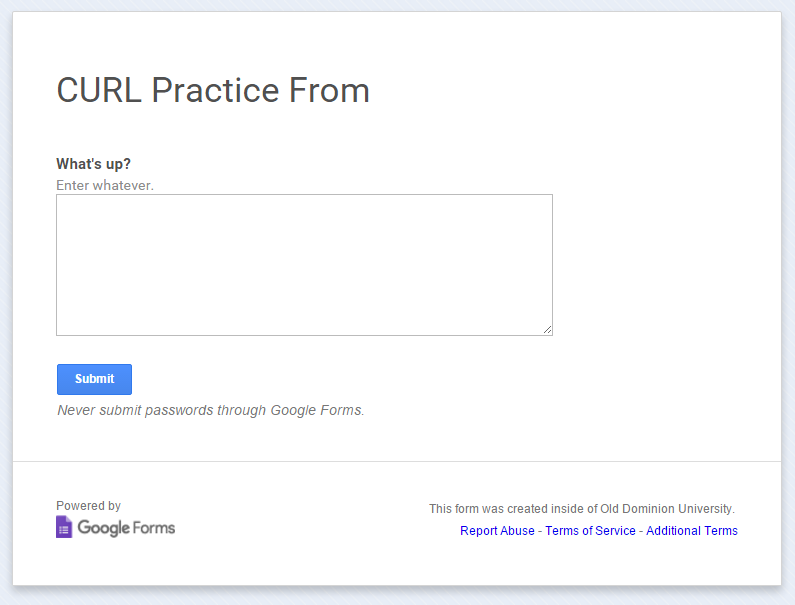
\includegraphics[width=5in]{GoogleForm.png}
\caption{Sample of my form}
\end{figure}
\newpage

From there I opened its source page, where I found the text box link by searching for the form and action tags. For this type of form, I also searched for the entry link.

\begin{figure}[h]
\centering
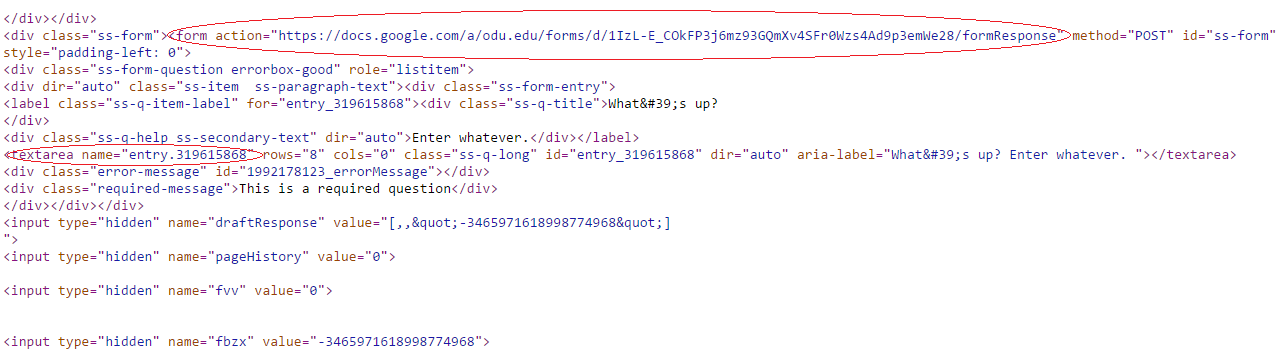
\includegraphics[width=7in]{FormSourceCode.png}
\caption{Part of the source code of my form page}
\end{figure}

Now I just use curl command with -i and -d options. The -i option requests for response from the page server and -d option posts my message on the form. Following the options are the entry link and my actions; after that is the text box link. The image below is just a screen capture of the response header, the full response is saved in a html file call post.html which I will provide in my github repository.

\begin{figure}[h]
\centering
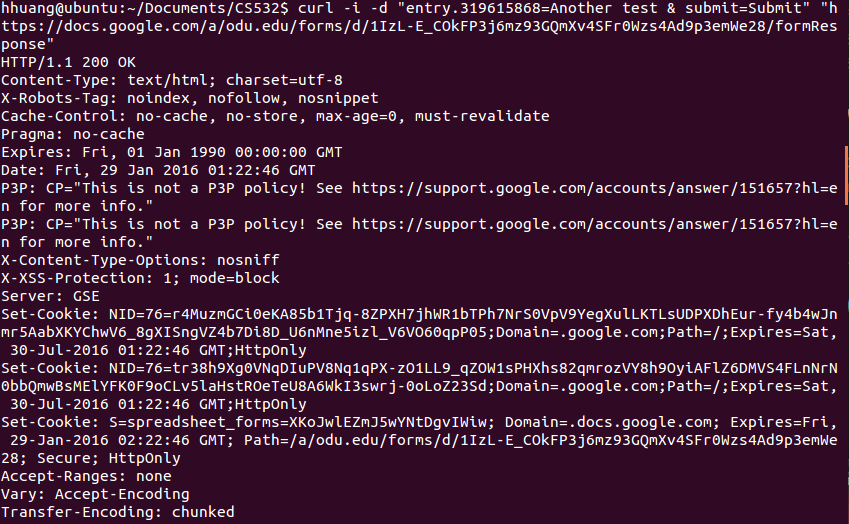
\includegraphics[width=5in]{PostResponse.png}
\caption{Response of my post}
\end{figure}

\newpage

Whatever message that was posted to the form is automatically saved to a spread sheet by Google. Here are the posts I made to the form.

\begin{figure}[h]
\centering
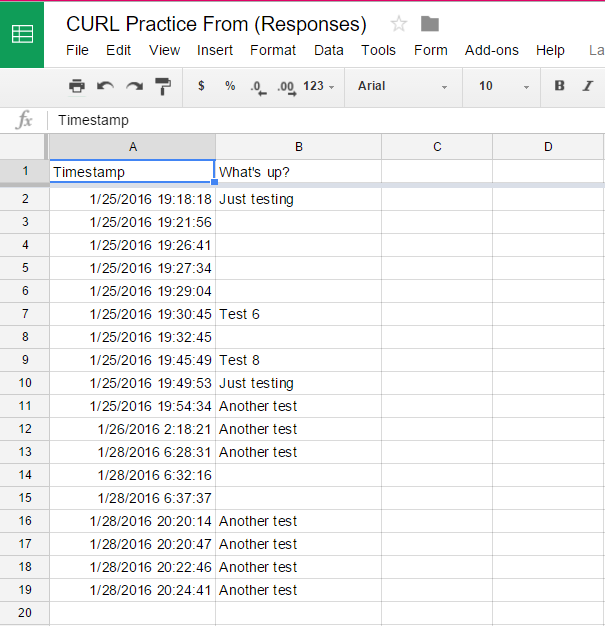
\includegraphics[width=5in]{FormPosts.png}
\caption{My posts}
\end{figure}
\newpage

\section*{Problem 2}
 Write a Python program that:\\
  1. takes as a command line argument a web page\\
  2. extracts all the links from the page\\
  3. lists all the links that result in PDF files, and prints out
     the bytes for each of the links.  (note: be sure to follow
     all the redirects until the link terminates with a "200 OK".)\\
  4. show that the program works on 3 different URIs, one of which
     needs to be: \\
     http://www.cs.odu.edu/~mln/teaching/cs532-s16/test/pdfs.html
     
\subsection*{Answer}

At this point, I would like to state that I received some help from my fellow class mate Zetan Li. He pointed me to a web page that made everything so much easier(\url{http://docs.python-requests.org/en/latest/api/#requests.Response}).

I used import sys to enable me to take command line argument of a web page. The web page url is assigned to the object named weburl, argument 1 is used because argument 0 is always preserved for the file name. I send a get request for the source information of the web page. Then I convert whatever I got from the get request into unicode and run them through beautifulsoup. From the result I find all ``a'' tag to get all the hyperlinks of the page and assign the result in object named links. Then, from the ``a'' tagged link results I get every ``herf'' links and for each one of them, call the function getHeader(). In this function, I use request.get command again, which is so helpful in this assignment. Because the get command with the request library will automatically chase down the redirected links until it receives a 200 ok code. Then, I use a if statement to isolate the links that have a content type of application/pdf in its response header. For the ones that fit all the criteria, program will print out the url link, response codes, and file size.

\newpage

The first web page I used to test against my program is: 
\url{http://www.cs.odu.edu/~mln/teaching/cs532-s16/test/pdfs.html}. From which my program found 10 url links that directed to pdf files.

\begin{figure}[h]
\centering
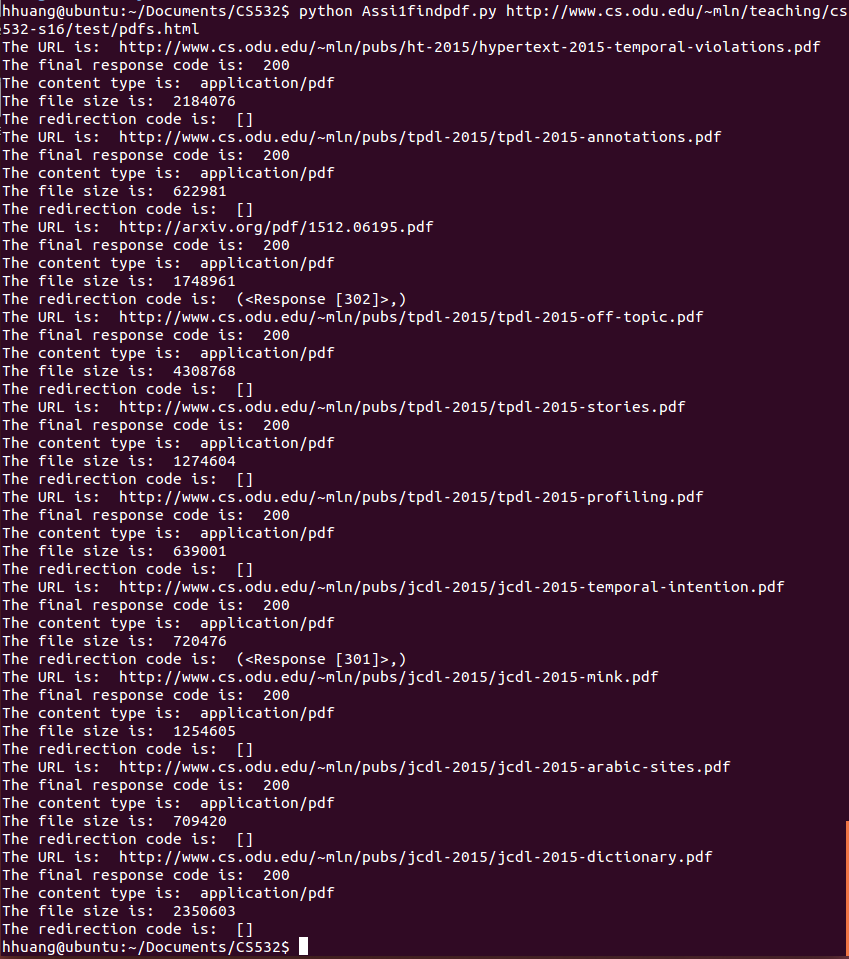
\includegraphics[width=5in]{web1.png}
\caption{The required web page}
\end{figure}
\newpage

The second web page I used to test against my program is: 
\url{http://www.cs.odu.edu/}. From which my program found 4 url links that directed to pdf files.

\begin{figure}[h]
\centering
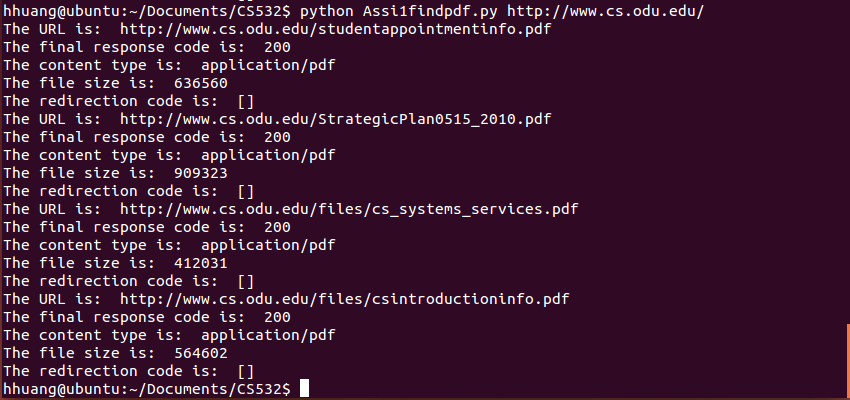
\includegraphics[width=5in]{web2.png}
\caption{ODU Computer Science Department main page}
\end{figure}

The last web page I used to test against my program is: 
\url{https://graduate.cs.odu.edu/ms/Getting_Started}. From which my program also found 4 url links that directed to pdf files.

\begin{figure}[h]
\centering
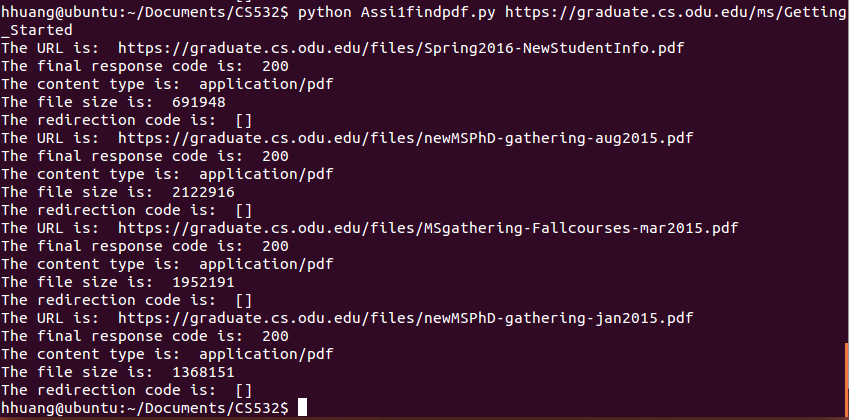
\includegraphics[width=5in]{web3.png}
\caption{Essential Resources page for ODU Computer Science Master degree students}
\end{figure}
\newpage

\section*{Problem 3}
Consider the "bow-tie" graph in the Broder et al. paper (fig 9):
    http://www9.org/w9cdrom/160/160.html
\noindent
Now consider the following graph:

\noindent
    A$\longrightarrow$B\\
    B$\longrightarrow$C\\
    C$\longrightarrow$D\\
    C$\longrightarrow$A\\
    C$\longrightarrow$G\\
    E$\longrightarrow$F\\
    G$\longrightarrow$C\\
    G$\longrightarrow$H\\
    I$\longrightarrow$H\\
    I$\longrightarrow$J\\
    I$\longrightarrow$K\\
    J$\longrightarrow$D\\
    L$\longrightarrow$D\\
    M$\longrightarrow$A\\
    M$\longrightarrow$N\\
    N$\longrightarrow$D\\
    O$\longrightarrow$A\\
    P$\longrightarrow$G\\
    
\noindent    
For the above graph, give the values for:\\
\noindent
    IN: \\
    SCC: \\
    OUT: \\
    Tendrils: \\
    Tubes: \\
    Disconnected:\\
\newpage

\subsection*{Answer}
For this problem, I first created a graph to help me decide the node types. 

\begin{figure}[h]
\centering
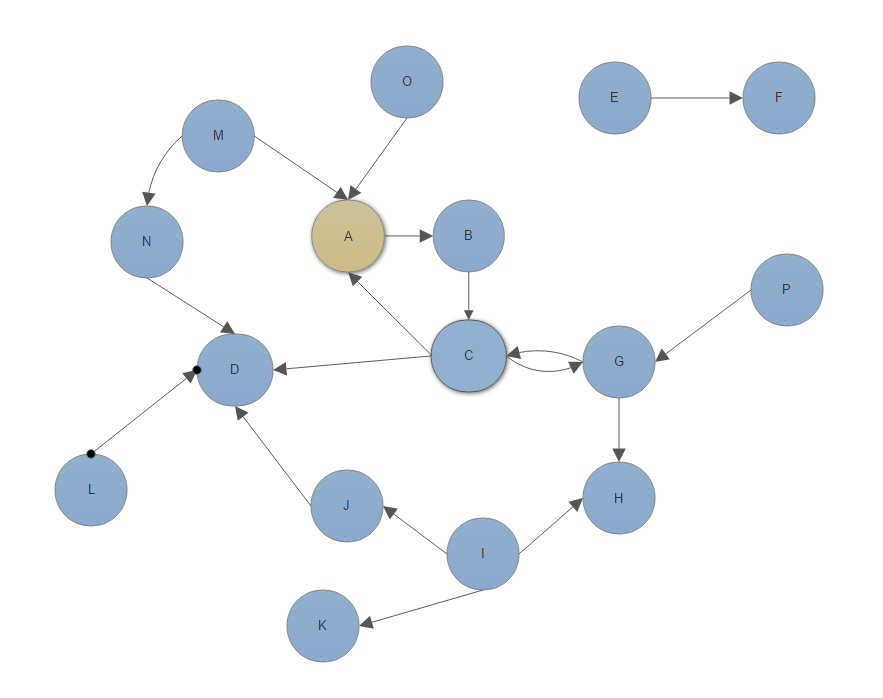
\includegraphics[width=5in]{Prablem3Graph}
\caption{Problem 3 Graph}
\end{figure}

\noindent
Now I apply the definitions of the node types:\\
IN: Nodes that only have links going out and connected directly to SCC nodes.\\
Out: Nodes that only have links going in and connected directly to SCC nodes.\\
SCC: Nodes that have links coming in from IN nodes and links going out to OUT nodes. Any SCC nodes can reach any other SCC nodes. \\
Tendrils: Nodes that are hanging from IN nodes or OUT node.\\
Tubes: Nodes that connect from IN to OUT without going through SCC.\\
Disconnected: Nodes that are not connected with main body of node networks.

\noindent
The node types according to the graph:\\
    IN: M \\
    SCC: A B C G\\
    OUT: D H\\
    Tendrils: I J K L O P\\
    Tubes: N\\
    Disconnected: E F\\

\end{document}